\chapter{Resultats}
\label{chap-results}

\section{État fondamental du calcium oxalate}
Les calculs numériques qui seront présentés dans cette section ont été faits avec \textit{Abinit}.

\subsection{Structure moléculaire}
La cellule élémentaire de calcium oxalate ($\V{Ca C_2 O_4}$) contient 28 atomes (cf.~\cite{Kolezynski2010}).
Il est de structure monoclique et de groupe de symétrie $P2/m$ ($\#$10) (cf. \cref{BrillouinZone})

\begin{figure}[!h]\label{BrillouinZone}
    \centering
    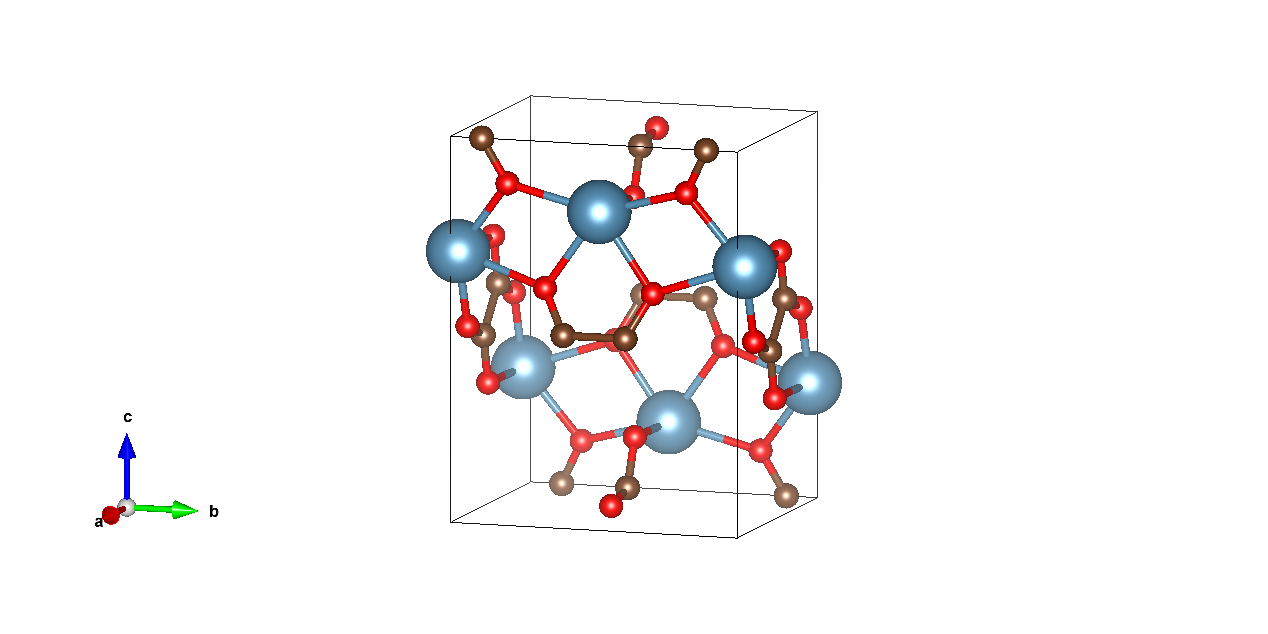
\includegraphics[width=20cm]{co_structure}
    \caption{La cellule élémentaire de l'oxalate de calcium}
\end{figure}
\subsection{Énergie de seuil}
D'abord, nous calculons la densité d'électrons de l'état fondamental
en fonctions des orbites de Kohn et Sham,
qui sont elles même représentées dans l'espace d'ondes plane tranché.
Pour chaque échantillonnage, l'énergie total du système dans l'état fondamental est calculé
en variant $E_{\V{cut}}$ (\cref{subsec-planewave}).
Le but du jeux est d'assurer la convergence du calcul en prenant le moins de fonctions d'onde possible.
On fait varier le seuil d'énergie $E_{cut}$ entre 20 et 100 Hatree.
On constate que pour tous ces seuils d'énergies, on obtient bien une convergence au bout de 15 itérations.
La relation entre l'énergie totale du système à la convergence
en fonction de l'énergie de seuil est tracée dans la \cref{fig-Ecut}.
À partir de $E_{cut} = 40$ Hatree, l'énergie totale du système est bien minimisée.
On choisit donc cette énergie de seuil pour la suite du calcul de l'état fondamental.

\begin{figure}[!h]\label{fig-Ecut}
    \centering
    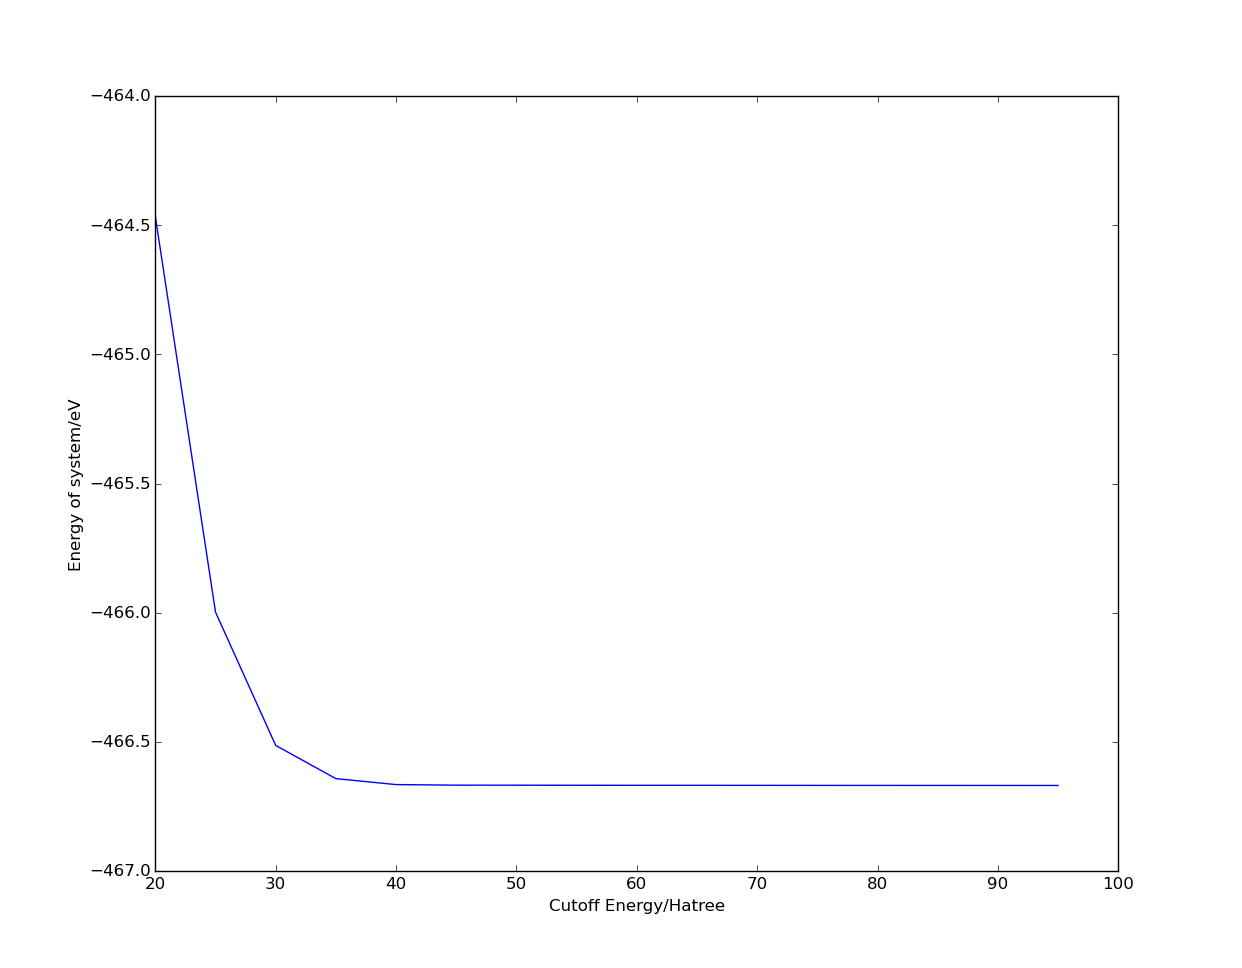
\includegraphics[width=12cm]{E_cut}
    \caption{Ecut}
\end{figure}

\section{Spectres de perte d'énergie (EELS)}
\subsection{Convergence avec les points-k: I}
Etant donnée la structure du système étudié et une fonction d'essai dont l'intégrale est facile à calculer,
Abinit peut nous donner une liste des échantillons avec pour chacun une valeur de présion
qui est définie par le calcul de l'intégral approximé sur l'ensemble de points $\vb{k}$ dans l'échantillon
par rapport au calcul exact.
La motivation de ce test de convergence est de pouvoir avoir un échantillonnage
assez fin pour obtenir tous les états d'excitation possibles sans avoir trop de points-k,
ce qui augmentera considérablement la compléxité du calcul.

La table \cref{tab-etotPK} montre que le système est déjà convergé avec peu de points-k (16) dans la première zone de Brillouin.
Ce résultat est dû au fait que la première zone de Brillouin est petite (car la maille élémentaire est grande).
\begin{table}[ht]\label{tab-etotPK}
\caption{Énergie totale du système en fonction du nombre de points-k}
\centering
\begin{tabular}{c c}
\toprule
Nombre de points-$\vb{k}$  &  $E_{tot}$ à la convergence (Hatree)
\\
\midrule
16    &  -466.66501448840
\\
28    &  -466.66501224916
\\
40    &  -466.66501098806
\bottomrule
\end{tabular}
\end{table}

\subsection{Approximation du potentiel d'échange et de corrélation}
Nous avons aussi examiné la qualité de l'approximation du potentiel d'échange et de corrélation
par la méthode LDA en la comparant avec la méthode GGA,
qui est censé être plus précise (cf. \cref{subsec-KS}).

Pour le cas de 16 points-k, nous avons obtenu la même valeur d'énergie totale pour les deux méthodes d'approximation.

\begin{table}[ht]\label{etotPK}
\caption{Énergie totale du système en fonction du nombre de points-$\vb{k}$}
\centering
\begin{tabular}{c c}
\toprule
Méthode d'approximation &  $E_{tot}$ à la convergence (Hatree)
\\
\midrule
LDA    &  -466.66501448840
\\
GGA   &   -466.66501448840
\bottomrule
\end{tabular}
\end{table}

Comme le nombre de points-k n'est pas élevé,
il est tout à fait possible que le résultat dépende peu de la méthode d'approximation
pour le terme d'échange et de corrélation.

Dans la suite, nous utiliserons ces résultats pour calculer la fonction diélectrique
dont on déduit les spectres de perte d'énergie d'électron (\cref{subsec-eels}).
\section{Spectres de perte d'énergie (EELS)}
Les calculs de cette section ont été fait avec le code de \textit{DP}.
L'objectif de cette section est de présenter les caractéritiques spectroscopiques
auxquelles on peut s'attendre dans une vraie expérience,
à l'aide des calculs \textit{ab initio}
\subsection{Convergence avec les points-k: II}
Même si les calculs de convergence avec les nombres de points-k différents ont été faits pour l'état fondamental,
il faut s'assurer que l'échantillonnage que l'on a privilégié soit aussi assez fin pour les calculs de réponse de la matériau sous une excitation extérieure.
On crée des fichiers décrivant la densité de l'état fondamental avec des échantillonnages
de la première zone de Brillouin différents,
où dans la première zone de Brouillin, il y a respectivement 16, 120 et 480 points-k.
Pour connaître le meilleur échantillonnage à utiliser à notre disposition,
on fait d'abord les calculs en prenant RPA (ramdom phase approximation)
comme méthode d'approximation du terme d'échange et de corrélation.
Pour le cas du calcium oxalate, nous avons choisi dans cette liste trois échantillons,
qui contiennent respectivement 16 (avec symétries),
120 (avec symétries) et 480 (grillage translaté et sans symétries) points $\vb{k}$.
%TODO: where is the kptCompare?
On montre dans la \cref{kptCompare} que le choix du 120 points-k dans la première zone de Brillouin
donne déjà de bons résultats pour le calcul de EELS (par rapport à 480 points-k).
On peut donc se contenter de prendre l'échantillonnage avec 120 points-k pour la suite du calcul.

\subsection{Convergence avec les bandes}

\begin{figure}[!h]\label{fig-cv_nbd}
    \centering
    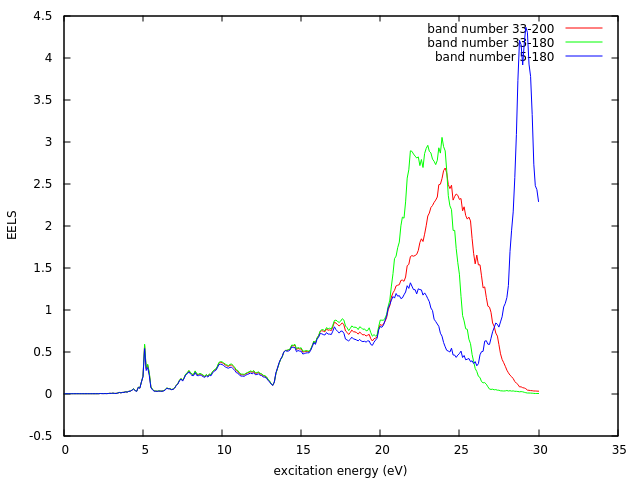
\includegraphics[width=12cm]{nbd_compare}
    \caption{Convergence en bande}
\end{figure}

Pour le calcul de $\epsilon^{-1}$ (l'inverse de la fonction diélectrique, qui servira à calculer EELS),
%TODO: where is TRL?
il faut passer par le calcul de la fonction de réponse linéaire (cf. \cref{TRL}).
Pour ce calcul, on doit considérer toutes les transitions possibles
(excitation d'un électron de la bande de valence vers une bande de conduction).
Il est donc nécessaire de converger le calcul de EELS par rapport au nombre de bandes de valence
et de conduction (cf. \cref{chi}).
Le but est de considérer seulement les transitions pour les énergies qui nous intéressent
afin de gagner en temps de calcul sans perdre des informations.
Nous nous intéressons notamment aux transitions en basse énergie (< 20 eV).
Le résultat montré dans la \cref{fig-cv_nbd} montre qu'il suffit de prendre en compte
les transitions entre la bande remplie numéro 33
(en comptant à partir de la bande d'énergie la plus basse) et la bande numéro 180.

\subsection{RPA vs ALDA}
La méthode d'approximation du terme d'échange et de corrélation RPA prend moins de temps
pour le calcul mais pourrait perdre la précision.
Il est donc judicieux de comparer les résultats obtenus en appliquant RPA avec ceux obtenus
en appliquant ALDA (adiabatic local density approximation).
Les deux approximations nous donnent des résultats assez proches en basses énergies.
Dans le cadre de ce projet, on se contente d'étudier les caractéristiques
de calcium oxalate en basse énergie en raison du délai.
Il est donc tout à fait pertinent de faire notre calcul en RPA pour gagner en temps de calcul.
\begin{figure}[!h]
    \centering
    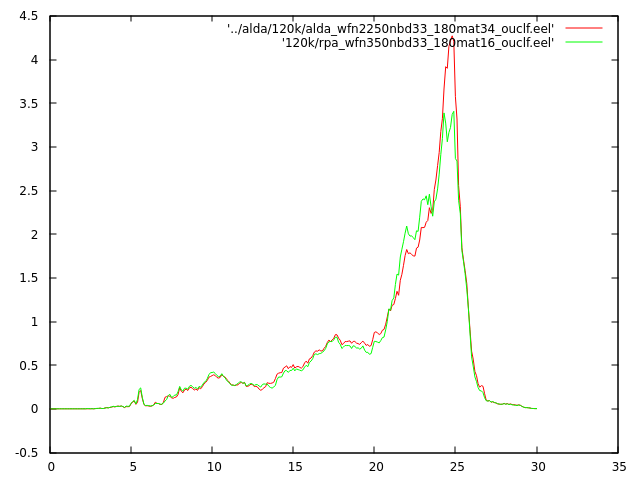
\includegraphics[width=8cm]{alda_vs_rpa}
    \caption{alda}
\end{figure}
\subsection{Anisotropie du système}

\begin{figure}[!h]\label{fig-anisotropie}
    \centering
    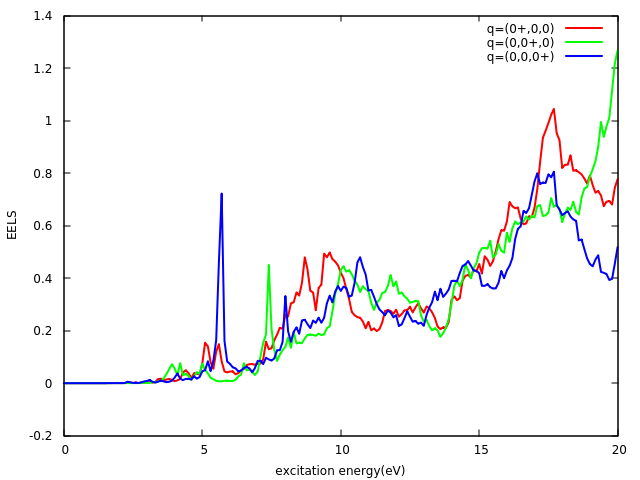
\includegraphics[width=12cm]{anisotropy}
    \caption{L'anisotropie du système}
\end{figure}

Cette étude consiste à examiner l'isotropie du système.
En effet, les transitions peuvent avoir lieu dans les directions différentes.
Un électron peut changer son vecteur d'onde en allant d'une bande à une autre.
Ce type de transition est pris en compte dans l'\cref{chi_q} qui nous donne la polarizabilité
que l'on est censé observer dans une direction donnée ($\vb{q}$ dans l'\cref{chi_q})
Or, comme certains termes sont négligés dans le calcul numérique,
on peut avoir des valeurs différentes en $q = 0$ en fonction de la direction par laquelle on s'y rapproche.
Les calculs de EELS en $\vb{q} = 0$ selon les trois axes
(par exemple, $\vb{q}=(0+,0,0)$ pour le premier axe de la zone de Brillouin)
sont montrés dans la \cref{fig-anisotropie}.
La différence entre les différentes valeurs trouvées est dûe à l'anisotropie de la structure.
%picture missing
\subsection{EELS et la fonction diélectrique}

\begin{figure}[!h]\label{fig-epsilon_compare}
    \centering
    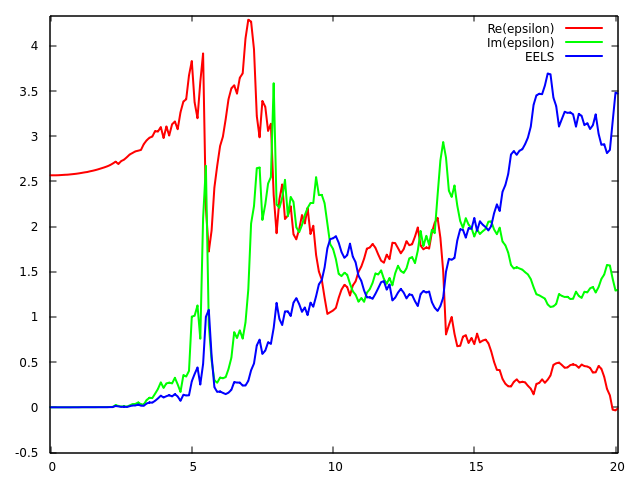
\includegraphics[width=12cm]{epsilon_compare}
    \caption{Relation entre les parties réelle et imaginaire de la fonction diélectrique $\epsilon$ et EELS}
\end{figure}

On se rappelle que la relation entre EELS et la fonction diélectrique est donnée par \cref{EELS}.
On peut constater que, dans la \cref{fig-epsilon_compare}, la partie de réelle et
la partie imaginaire de la fonction diélectrique ont des sens de croissance opposés.
On pourrait donc s'attendre à un pic de résonance de EELS à l'endroit où elles se croisent
(aux alentours de 5 eV).
Ensuite, les deux parties prennent des valeurs bien supérieures à zéro,
la croissance de EELS dépend cette fois-ci plus de la partie imaginaire de la fonction diélectrique.
Le continuum du spectre pour le régime d'énergie supérieure à 7 eV est dû au fait
qu'il n'y a pas de croisement entre les parties réelle et imaginaire à valeur près de zéro.

\subsection{Dispersion}
Enfin, on s'intéresse à la dispersion des spectres EELS\@.
Il s'agit de changer la valeur de $\vb{q}$ dans l'\cref{chi_q} (non proche de 0 cette fois-ci).
Il est intéressant de remarquer que la stabilité de la position du premier pique de résonance
pour les trois différentes directions de dispersion (\cref{fig-q6, fig-q8, fig-q10}).
Bien que la valeur de EELS obtenue pour le premier pique change en fonction de $\vb{q}$,
le pique se trouve toujours en même énergie d'excitation
quand on fait varier la valeur de $\vb{q}$ dans une direction donnée.

Dans une vraie expérience, on est limité par la résolution des l'appareils.
Il est donc difficile à déterminer, en général, si une réponse forte est due
à une résonance ou à une superposition de réponses pour différentes valeurs de $\vb{q}$.
Pour l'oxalate de calcium, un expérimentateur pourra se convaincre que la réponse qu'il obtiendra
pour une énergie qui correspond à un pique de EELS est une vraie résonance.


\begin{figure}[!h]\label{fig-q6}
    \centering
    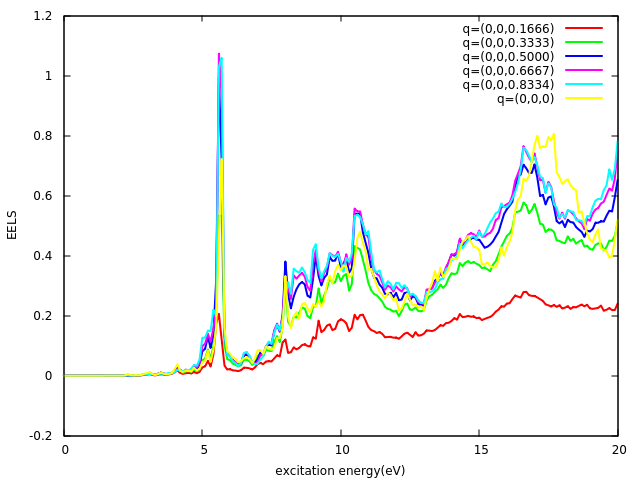
\includegraphics[width=12cm]{q6}
    \caption{EELS pour différents $\vb{q}$ dans la direction (0, 0, 1) de la première de Brillouin}
\end{figure}

\begin{figure}[!h]\label{fig-q8}
    \centering
    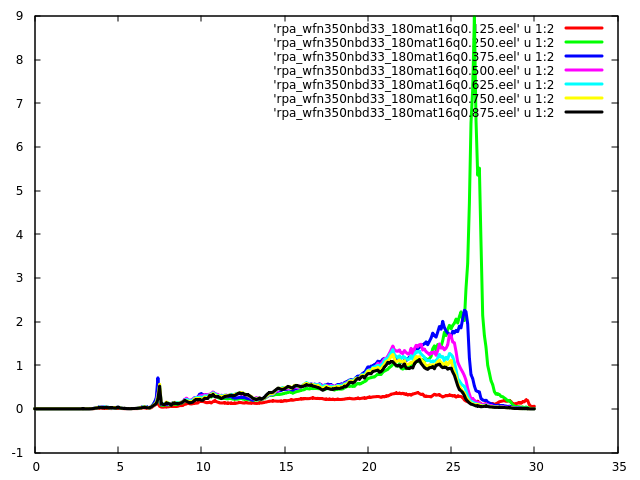
\includegraphics[width=12cm]{q8}
    \caption{EELS pour différents $\vb{q}$ dans la direction (0, 1, 0) de la première de Brillouin}
\end{figure}
\begin{figure}[!h]\label{fig-q10}
    \centering
    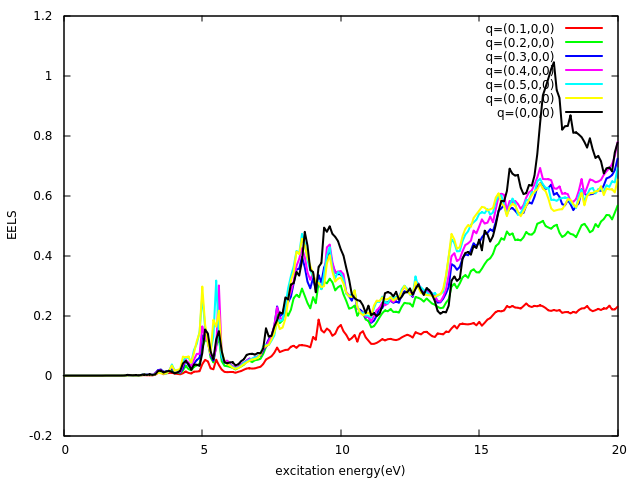
\includegraphics[width=12cm]{q10}
    \caption{EELS pour différents $\vb{q}$ dans la direction (1, 0, 0) de la première de Brillouin}
\end{figure}
